% -*- TeX-master: "Slides.tex" -*-


\PassOptionsToPackage{dvipsnames, table}{xcolor}
\documentclass{beamer}
% \documentclass[draft]{beamer}


\usepackage[utf8]{inputenc}
\usepackage[T1]{fontenc}
\usepackage{lmodern}
\usepackage[english]{babel}
\usepackage{svg}
\usepackage{caption, subcaption}
\usepackage{amsmath, amssymb}
\usepackage{booktabs}

\usepackage[backend=biber, style=alphabetic]{biblatex}


\usepackage[nomain, nolangwarn, savewrites]{glossaries}
\setupglossaries{
  toc,
  shortcuts,
  ucmark,
  nogroupskip
}
\setglossarysection{section}
% \setglossarystyle{longragged3col-booktabs}
\DeclareAcronymList{main, models}
\newglossary*{main}{Primary}
\newglossary*{models}{Models}
\makeglossaries
% -*- TeX-master: "Thesis.tex" -*-


% Deep Learning related.
\newacronym{ann}{ANN}{Artificial Neural Network}
\newacronym{dnn}{DNN}{Deep Neural Network}
\newacronym{cnn}{CNN}{Convolutional Neural Network}
\newacronym{rnn}{RNN}{Recurrent Neural Network}
\newacronym{nlp}{NLP}{Natural Language Processing}
\newacronym{relu}{ReLU}{Rectified Linear Unit}
\newacronym{lstm}{LSTM}{Long Short Term Memory}
\newacronym{gru}{GRU}{Gated Recurrent Unit}
\newacronym{bptt}{BPTT}{Backpropagation Through Time}
\newacronym{cv}{CV}{Computer Vision}
\newacronym{ai}{AI}{Artificial intelligence}

% Related to thesis topic.
\newacronym{re}{RE}{Referring Expression}
\newacronym{rec}{REC}{Referring Expression Comprehension}
\newacronym{iou}{IoU}{Intersection over Union}

% Basic.
\newacronym{iff}{iff}{if and onnly if}
\newacronym{sota}{SOTA}{state of the art}
\newacronym{rgb}{RGB}{Red, Green and Blue}
\newacronym{iot}{IoT}{Internet of Things}

% Loss functions.
\newacronym{ce}{CE}{Cross Entropy}
\newacronym{wce}{WCE}{Weighted Cross Entropy}
\newacronym{bce}{BCE}{Balanced Cross Entropy}
\newacronym{fl}{FL}{Focal Loss}
\newacronym{dnc}{DNC}{Distance to the Nearest Cell}
\newacronym{dc}{DC}{Dice Coefficient}
\newacronym{dl}{DL}{Dice Loss}
\newacronym{ti}{TI}{Tversky Index}



\colorlet{rowColor}{gray!10}
\colorlet{topRowColor}{gray!37.5}
\definecolor{blueGantt}{HTML}{0066FF}
\definecolor{greenGantt}{HTML}{33CC33}
\definecolor{yellowGantt}{HTML}{FFFFCC}



\renewcommand{\arraystretch}{1.25}


\newcommand*{\re}[1]{\textsf{#1}}
\newcommand*{\code}[1]{\texttt{#1}}


\addbibresource{Utils/References.bib}




\newcommand{\R}{\mathbb{R}}
\newcommand{\loss}{\mathcal{L}}

\DeclareMathOperator*{\argmin}{arg\,min}


\usepackage{tikz, pgfplots, pgfgantt}




% Tikz configuration.
\usetikzlibrary{
  external,
  positioning,
  fit,
  backgrounds,
  arrows,
  shadows.blur,
  calc,
  shapes.geometric
}
\tikzexternalize[prefix=Build/Tikz/, figure name=FigureSlide]

% Pgfplots configuration.
\pgfplotsset{compat=newest}
\usepgfplotslibrary{external}
\pgfplotsset{%
  activationFunction/.style = {%
    xlabel = {$x$}, ylabel = {$y$},
    legend style = {
      at = {(0.5, 1.05)},
      anchor = south,
    },
    grid = both,
    xtick distance = 1, ytick distance = 1,
    minor tick num = 1,
    major grid style = {thin, dashed, gray!60},
    minor grid style = {thin, dashed, gray!20},
    axis lines = center,
    axis line style = {
      very thick,
      -latex
    },
    enlargelimits,
    width = \textwidth,
    scale only axis,
  },
  trainPlot/.style = {
    width = \textwidth,
    height = .5\textwidth,
    grid = major,
    grid style = {dashed, gray!40},
    xlabel = {Epoch number},
    thick,
    legend pos = north east,
  }
}




% Configuration for SVG package.
\svgsetup{
  inkscapepath = Build/SVG/
}
\svgpath{Figures/}

% Set path for figures (relative to main document).
\graphicspath{{./Figures/}}

% \setbeameroption{show notes} % Comentar/Descomentar para las notas
\usetheme{CambridgeUS}
\usecolortheme{orchid}
\setbeamercolor{titlelike}{parent=structure, bg=gray!15}
\setbeamercovered{transparent}

\AtBeginSection[]{
  \begin{frame}{Chapter Outline}
    \tableofcontents[currentsection, sectionstyle=show/hide, subsectionstyle=show/show/hide]
  \end{frame}
}


\title[Referring Expression Comprehension]{
  Exploring and Visualizing\\
  Referring Expression Comprehension}
\subtitle{Bachelor's Thesis (Mathematics \& Industrial Engineering)}

\author[David Álvarez Rosa]{
  David Álvarez Rosa\inst{1,2,3}\\
  \and
  \textsl{Supervisor:} Sanja Fidler\inst{5}
  \and
  \textsl{Co-Supervisor:} Xavier Giró\inst{4}
}
\institute[UPC]{
  Politechnical University of Catalonia\\
  {\tiny
  \inst{1}Interdisciplinary Higher Education Centre\\
  \inst{2}Barcelona School of Industrial Engineering ---
  \inst{3}School of Mathematics and Statistics\\
  \inst{4}Signal Theory and Communications Department}
  \and
  University of Toronto\\
  {\tiny
  \inst{5}Computer Science Department}
}

\logo{
  \includesvg[height=1cm]{Logos/UofT.svg}
  \hspace{1.5em}
  \includesvg[height=1cm]{Logos/UPC.svg}
}

\date{Barcelona -- \today}



\begin{document}

\section*{Front Matter}

\subsection{Title}

\begin{frame}
  \titlepage
\end{frame}


\subsection{Acknowledgments}

\begin{frame}{Acknowledgments}
  Acknowledgments.
\end{frame}


\subsection{Table of Contents}

\begin{frame}{Table of Contents}
  \tableofcontents[hideallsubsections]
\end{frame}



\section{Chapter 1. Introduction}

\subsection{Description and Motivation}

\begin{frame}{Problem Description}{Referring Expression Comprehension}
  Image\onslide<2->{ + Referring Expression}\onslide<3>{ \(\longrightarrow\) Segmentation!}
  \begin{figure}
    \begin{subfigure}[t]{.32\textwidth}
      \onslide<2->{\caption{Man with cap}}
      \includegraphics<1-2>[width=\textwidth]{Images/Man with cap (COCO).jpg}%
      \includegraphics<3>[width=\textwidth]{Images/Man with cap.jpg}
    \end{subfigure}\hfill
    \begin{subfigure}[t]{.32\textwidth}
      \onslide<2->{\caption{Laptop on the right}}
      \includegraphics<1-2>[width=\textwidth]{Images/Laptop on the right (COCO).jpg}%
      \includegraphics<3>[width=\textwidth]{Images/Laptop on the right.jpg}
    \end{subfigure}\hfill
    \begin{subfigure}[t]{.32\textwidth}
      \onslide<2->{\caption{Army officer white suit}}
      \includegraphics<1-2>[width=\textwidth]{Images/Army officer (COCO).jpg}%
      \includegraphics<3>[width=\textwidth]{Images/Army officer.jpg}
    \end{subfigure}
    \caption{Examples of Referring Expression Comprehension}
  \end{figure}
\end{frame}

\begin{frame}{Big Frame}{Referring Expression Comprehension}
  \begin{columns}
    \begin{column}{.5\textwidth}
      \centering
      \includegraphics<1>[width=.7\textwidth]{Images/AI, ML and DL.png}
      \includegraphics<2->[width=.75\textwidth]{Images/Computer Vision.jpg}
      \only<3>{{\\{\Huge +}\\}}
      \includegraphics<2->[width=.45\textwidth]{Images/Natural Language Processing.png}
    \end{column}

    \begin{column}{.5\textwidth}
      Regarding learning \alert{techniques}
      \begin{itemize}
        \item Artificial Intelligence
        \item Machine Learning
        \item Deep Learning
      \end{itemize}
      \pause
      Regarding \alert{type} of data
      \begin{itemize}
        \item Computer Vision
        \item Natural Language Processing
        \pause
        \item \ldots{} and Multimodal Learning
      \end{itemize}
    \end{column}
  \end{columns}
\end{frame}

\begin{frame}{Objectives}{Bachelor's Thesis}
  \begin{itemize}
    \item Learning about Machine Learning (ML)
    \item Fundamentals of neural models
    \item Undestand state-of-the-art papers
    \item Model (in REC and Speech to Text)
    \item Front end development (HTML, CSS, JS)
    \item Back end (PHP)
    \item Academia (creationg of thesis and presentation)
  \end{itemize}
\end{frame}


\subsection{Applications}

\begin{frame}{Applications}{Referring Expression Comprehension}
  \begin{columns}
    \begin{column}{.5\textwidth}
      \centering
      \includegraphics[width=.75\textwidth]{Images/Robot.jpg}\\
      \medskip
      \includegraphics[width=.75\textwidth]{Images/Robots.png}
    \end{column}

    \begin{column}{.5\textwidth}
      \begin{itemize}
        \item Theoretical
        \item Industry
        \item Home Automation and IoT
        \item Security
      \end{itemize}
    \end{column}
  \end{columns}
\end{frame}



\section{Chapter 2. Theoretical Background}

\subsection*{}

\begin{frame}[t]{Machine Learning Overview}{From Reality to Fiction}
  \begin{block}{Mathematical perspective}
    Given dataset \(\Omega\) of inputs \(x \in \R^n\) and outputs
    \(y \in \R^m\), find
    \begin{equation}
      \begin{aligned}
        f \colon \R^n &\longrightarrow \R^m\\
        x &\longmapsto f(x) := \hat{y},
      \end{aligned}
    \end{equation}
    such that \(\hat{y} \approx y\) for every element in the dataset.
  \end{block}
  \pause
  \begin{alertblock}{Desired generalization}
    We do not seek memorization, we seek to extract relevant information from
    the structure of the data in order to make \alert{predictions}.
  \end{alertblock}
\end{frame}


\subsection{Tensors}

\begin{frame}{Tensors}{View as multidimensional arrays}
  \begin{columns}
    \begin{column}{.5\textwidth}
      \begin{figure}
        \includegraphics[width=\textwidth]{Images/Tensor.png}
        \caption{Tensor representation}
      \end{figure}
    \end{column}
    \begin{column}{.5\textwidth}
      \begin{itemize}
        \item We will understand the tensors as a grouping data structure,
        \item i.e, as multidimensional arrays.
        \item \(T_i\), with index \(i = (i_1, \ldots, i_n)\)
      \end{itemize}
      \begin{exampleblock}{Tensor example}
        Images as tensor of rank 3,
        \begin{equation}
          I \in \R^{C \times H \times W}.
        \end{equation}
      \end{exampleblock}
    \end{column}
  \end{columns}
\end{frame}


\subsection{Neural Network Architectures}

\begin{frame}{Neural Network Architectures}{Overview}
  \begin{itemize}
    \item Feedforward Neural Network
    \item Convolutional Neural Network
    \item Recurrent Neural Network
    \item Transformer Model
  \end{itemize}
\end{frame}

\begin{frame}{Feedforward Neural Network}{Topology: Layers, Neurons and Connections}
  \begin{figure}
    \input{Figures/Tikz/Fully Connected Neural Network.tex}
    \caption{Feedforward Neural Network architecture}
  \end{figure}
\end{frame}

\begin{frame}{Feedforward Neural Network}{Mathematical Representation}
  \begin{block}{Forward computation}
    The output values are \(y = x^L\) can be computed recursively,
    \begin{equation}
      x^{\ell+1} = f\left(W^\ell x^\ell + b^\ell\right),
    \end{equation}
    where \(W^l\) and \(b^l\) are a matrix and a vector of weights
    respectively.
  \end{block}
  \begin{exampleblock}{Example of digit recognition}
    \centering
    \includegraphics[width=.5\textwidth]{Images/MNIST.png}
  \end{exampleblock}
\end{frame}

\begin{frame}{Convolutional Neural Network}{Topology}
  \begin{figure}
    \includegraphics[width=\textwidth]{Images/Architecture LeNet-5.png}
    \caption{Convolutional Neural Network architecture}
  \end{figure}
\end{frame}

\begin{frame}{Convolutional Neural Network}{Convolutional Layer}
  \begin{columns}
    \begin{column}{.5\textwidth}
      \begin{figure}
        \includegraphics[width=\textwidth]{Images/Convolution.png}
        \caption{Convolution}
      \end{figure}
    \end{column}
    \begin{column}{.5\textwidth}
      \begin{block}{Mathematical definition}
        Given filter \(F\), the convolution is defined as follows,
        \begin{equation}
          Y_{i,j,k} = \sum_{l, m, n} X_{l, j + m, k + n} F_{i, l, m, n},
        \end{equation}
        where the sum is performed for all valid \(l, m, n\) indices.
      \end{block}
    \end{column}
  \end{columns}
\end{frame}

\begin{frame}{Convolutional Neural Network}{Pooling Layer}
  \begin{columns}
    \begin{column}{.5\textwidth}
      \begin{figure}
        \includegraphics[width=\textwidth]{Images/Max pooling.png}
        \caption{Max pooling}
      \end{figure}
    \end{column}
    \begin{column}{.5\textwidth}
      \begin{itemize}
        \item Reduce network dimension
        \item Add non-linearities
        \item Enlarge field of view
      \end{itemize}
      \begin{block}{Max pooling}
        \begin{equation}
          f_{X, Y}(S) = \max_{a, b=0}^1 S_{2X + a, 2Y + b}
        \end{equation}
      \end{block}
    \end{column}
  \end{columns}
\end{frame}

\begin{frame}{Recurrent Neural Network}{Topology}
  \begin{figure}
    \begin{subfigure}[t]{.2\textwidth}
      \centering
      \caption{Folded}
      \includegraphics[height=4cm]{Images/RNN.png}
    \end{subfigure}\hfill
    \begin{subfigure}[t]{.8\textwidth}
      \centering
      \caption{Unfolded}
      \includegraphics[height=4cm]{Images/Unfolded RNN.png}
    \end{subfigure}
    \caption{Recurrent Neural Netowrk architecture}
  \end{figure}
\end{frame}

\begin{frame}{TODO}{TODO}
  Quizá comentar aquí lo de LSTM y GRU.
  Y quizás añadir también la fórmula.
\end{frame}

\begin{frame}{Transformer Model}{Subtitle}
  TODO. Entender esto
  \includegraphics[width=\textwidth]{Images/Attention.png}
  \includegraphics[height=\textwidth]{Images/Transformer.png}
\end{frame}


\subsection{Training}

\begin{frame}{Training overview}{Loss functions}
  \begin{itemize}
    \item Measures differences between desired and predicted
    \item Dataset \(\Omega = {\{(x_i, y_i)\}}_{i=1}^N\)
    \item And, predicted output \(\hat{y} = f(x)\)
    \item It is common that,
    \begin{equation}
      \loss(\Omega, \theta) =
      \frac{1}{N} \sum_{(x, y) \in \Omega} \ell (x, y, \theta).
    \end{equation}
    \item We will assume \(\ell \in \mathcal{C}^1\)
  \end{itemize}
\end{frame}

\begin{frame}{Optimization}{Overall idea}
  \begin{itemize}
    \item We will seek to approximate,
    \begin{equation}
      \hat{\theta} = \argmin_{\theta} \loss(\Omega, \theta),
    \end{equation}
    given that the above exists.
    \item Usually iterative methods, i.e., given initial guess
    \(\theta^{(0)}\), proceed as follows,
    \begin{equation}
      \theta^{(t + 1)} = \theta^{(t)} + \alpha\,\Delta\theta^{(t)},
    \end{equation}
    where \(\alpha\) is called the step size (or learning rate), and
    \(\Delta\theta^{(t)}\) is the weight update in step \(t\).
  \end{itemize}
\end{frame}

\begin{frame}{Optimization}{Methods}
  \begin{itemize}
    \item First order methods (higher order infeasible)
    \item Gradient Descent:
    \begin{equation}
      \Delta\theta^{(t)} = -\nabla\loss(\theta^{(t)}).
    \end{equation}
    Due to loss function,
    \begin{equation}
      \nabla_{\theta}\,\loss(\Omega, \theta) =
      \frac{1}{N} \sum_{(x, y) \in \Omega} \nabla_{\theta}\,\ell (x, y, \theta).
    \end{equation}
    \item Therefore, in practice, \alert{Stochastic} Gradient Descent,
    \begin{equation}
      \nabla_{\theta}\,\loss(\Omega, \theta) \approx
      \frac{1}{\lvert B\rvert} \sum_{(x, y) \in B} \nabla_{\theta}\,\ell (x, y, \theta).
    \end{equation}
  \end{itemize}
\end{frame}

\begin{frame}{Optimization}{Methods II}
  \begin{alertblock}{Avoid saddle points}
    Using momentum,
    \begin{equation}
      \Delta\theta^{(t)} =
      -\beta\Delta\theta^{(t-1)} -\nabla\loss(\theta^{(t)}),
    \end{equation}
    where \(\beta\) is the ``friction'' hyperparameter.
  \end{alertblock}
\end{frame}

\begin{frame}{Optimization}{Weight initialization}
  \begin{itemize}
    \item Random
    \item Xavier initialization
  \end{itemize}
\end{frame}

\begin{frame}{Optimization}{Computing derivatives: error backpropagation}
  \begin{block}{Backpropagation algorithm exemplified}
    Let \(w_ {ij} ^ l\) be an individual weight, involved in computing
    \(\hat{y}_i^l\) then the \alert{chain rule} applied to
    \(\ell (x, y, \theta)\) yields,
    \begin{equation}
      \frac{\partial \ell}{\partial w_{ij}^l} =
      \frac{\partial \ell}{\partial \hat{y}_i^l}
      \frac{\partial y_i^l}{\partial w_{ij}^l}.
    \end{equation}
  \end{block}
  \begin{center}
    \resizebox{.6\textwidth}{!}{
      \input{Figures/Tikz/Fully Connected Neural Network.tex}
    }
  \end{center}
\end{frame}

\begin{frame}{Regularization Techniques}{Understanding overfitting}
  \begin{figure}
    \includegraphics[width=.65\textwidth]{Images/Overfit.png}
    \caption{Representation of the overfitting phenomenon}
  \end{figure}
\end{frame}

\begin{frame}{Regularization Techniques}{Avoiding overfitting}
  \begin{block}{\(L_2\) regularization}
    Add a term to loss function, i.e,
    \begin{equation}
      \hat{\loss}(\Omega, \theta) =
      \loss(\Omega, \theta) + \lambda\,\text{complexity}(\theta),
    \end{equation}
    where \(\lambda\) is the regularization hyperparameter, and,
    \begin{equation}
      \text{complexity}(\theta) = \lVert\theta\rVert_2^2 = \sum_{w \in \theta} w^2.
    \end{equation}
  \end{block}
\end{frame}

\begin{frame}{Regularization Techniques}{Avoiding overfitting II}
  \begin{itemize}
    \item Early stopping
    \begin{figure}
      \includegraphics[width=.45\textwidth]{Images/Early stopping.jpg}
    \end{figure}
    \item Data augmentation
  \end{itemize}
\end{frame}


\subsection{Testing}

\begin{frame}{Testing concept}{Save data to evaluate}
  \begin{itemize}
    \item Evaluate model
    \begin{itemize}
      \item Quantiative metrics
      \item Qualitative
    \end{itemize}
    \item Compare with state of the art
  \end{itemize}
  \begin{alertblock}{False evaluation metrics}
    Never train with \texttt{test} split!
  \end{alertblock}
\end{frame}



\section{Chapter 3. Referring Expression Comprehension}

\subsection{Problem Formulation}

\begin{frame}{Referring Expression Comprehension}{Reminder}
  \begin{columns}
    \begin{column}{.5\textwidth}
      \begin{figure}
        \includegraphics[width=\textwidth]{Images/Parent.jpg}
        \caption{Parent holding umbrella}
      \end{figure}
    \end{column}
    \begin{column}{.5\textwidth}
      \begin{itemize}
        \item Input 1: Image
        \item Input 2: Referring Expression
        \item Output: Segmentation
      \end{itemize}
    \end{column}
  \end{columns}
\end{frame}


\subsection{Training}

\begin{frame}{Datasets}{Subtitle}
  \begin{itemize}
    \item RefCOCO
    \begin{itemize}
      \item Generated from MS COCO dataset with a two-player game
      \item 142,209 samples (in 19,994 images)
    \end{itemize}
    \item RefCOCO+
    \begin{itemize}
      \item \alert{Location} information disallowed
      \item Similar size
    \end{itemize}
    \item RefCOCOg
    \begin{itemize}
      \item Only non-trivial elements
      \item 104,560 samples (in 26,711 images)
    \end{itemize}
    \item CLEVR-REF+
    \begin{itemize}
      \item Images generated synthetically (data augmentation)
    \end{itemize}
  \end{itemize}
\end{frame}

\begin{frame}{Loss Functions}{Cross entropy}
  The ``difference'' between predicted and ground truth pixels is computed as,
  \begin{equation}
    \text{\acs{ce}}(p, \hat{p}) = -(p\log\hat{p} + (1 - p)\log(1 - \hat{p})).
  \end{equation}
  \begin{exampleblock}{Intuitive interpretation}
    Taking into account that \(p \in \{0, 1\}\), the loss function can be
    rewritten as follows,
    \begin{equation}
      \text{\acs{ce}}(p, \hat{p}) =
      \begin{cases}
        -\log(1 - \hat{p}) & p = 0 \\
        -\log\hat{p} & p = 1.
      \end{cases}
    \end{equation}
  \end{exampleblock}
\end{frame}

\begin{frame}{Loss Functions}{Cross entropy variants}
  Modifying cross entropy:
  \begin{itemize}
    \item \acf{wce}
    \begin{equation}
      \text{\acs{wce}}(p, \hat{p}) =
      -(\beta p\log\hat{p} + (1 - p)\log(1 - \hat{p})).
    \end{equation}
    \item \acf{bce}
    \begin{equation}
      \text{\acs{bce}}(p, \hat{p}) =
      -(\beta p\log\hat{p} + (1 - \beta)(1 - p)\log(1 - \hat{p})).
    \end{equation}
  \end{itemize}
\end{frame}

\begin{frame}{Loss Functions}{Intersection over Union or Jaccard Index}
  \begin{columns}
    \begin{column}{.5\textwidth}
      \centering
      \includegraphics[width=.7\textwidth]{Images/Object detection Bounding Boxes.jpg}\\[1ex]
      \includegraphics[width=.7\textwidth]{Images/Intersection over Union.png}
    \end{column}
    \begin{column}{.5\textwidth}
      \begin{block}{Mathematical definition}
        Given the predicted segmentation \(A\) and the ground truth \(B\), the
        Jaccard index is defined as follows,
        \begin{equation}
          J(A,B) = \frac{|A \cap B|}{|A \cup B|}.
        \end{equation}
      \end{block}
    \end{column}
  \end{columns}
\end{frame}

\begin{frame}{Loss Functions}{Dice Loss}
  \begin{alertblock}{Intersection over Union as loss function?}
    Cannot be used directly as a loss function since optimization will be
    \alert{infeasible} (think about non-overlapping bounding boxes).
  \end{alertblock}
  So, we define, \acf{dil} as folows,
  \begin{equation}
    \text{\acs{dil}}(p, \hat{p}) = 1 -
    \frac{2\sum p_{h, w}\hat{p}_{h, w}}{\sum p_{h, w} + \sum \hat{p}_{h, w}}.
  \end{equation}
\end{frame}

\begin{frame}{Loss Functions}{And much more}
  \begin{figure}
    \includegraphics[width=.85\textwidth]{Images/Loss.png}
    \caption{Overview of loss functions}
  \end{figure}
\end{frame}


\subsection{Evaluation Techniques}

\begin{frame}{Quantitative Measures}{Derived from Intersection over Union}
  \begin{itemize}
    \item Overall IoU, defined as,
    \begin{equation}
      \text{Overall \gls{iou}} =
      \frac{\sum_{i=0}^N I_i}{\sum_{i=0}^n U_i},
    \end{equation}
    where \(I_i\) and \(U_i\) correspond to the \(i\)-th intersection and union
    (respectively) between the prediction and the ground truth.
    \item Mean IoU, defined as,
    \begin{equation}
      \text{\Acl{miou}} = \frac{1}{N}\sum_{i=0}^N \text{\gls{iou}}_i.
    \end{equation}
    \item Precision at Threshold: judge as true/false positive using the
    \gls{iou}.
  \end{itemize}
\end{frame}

\begin{frame}{Qualitative Evaluation}
  \begin{itemize}
    \item Analyze with your eyes
    \item Be smart
    \item Not numeric but useful
  \end{itemize}
\end{frame}


\subsection{Related Work}

\begin{frame}{Multimodal Embedding}{Joint space}
  \begin{figure}
    \includegraphics[width=.75\textwidth]{Images/Joint.png}
    \caption{Multimodal embedding visual-semantic space}
  \end{figure}
\end{frame}

\begin{frame}{Modular Models}{Models}
  \begin{figure}
    \includegraphics[width=.75\textwidth]{Images/MattNet.png}
    \caption{Modular Attention Network (MAttNet)}
  \end{figure}
\end{frame}

\begin{frame}{Graph Generation}{Models}
  \begin{figure}
    \includegraphics[width=.75\textwidth]{Images/Graph model.png}
    \caption{Summary representation of graph-based models}
  \end{figure}
\end{frame}



\section{Chapter 4. Models}

\subsection{Referring Expression Comprehension}

\begin{frame}{Base Architecture}{Topology}
  \begin{figure}
    \includegraphics[width=\textwidth]{Images/RefVOS.png}
    \caption{Referring Expression for Video Object Segmentation (RefVOS)}
  \end{figure}
\end{frame}

\begin{frame}{Base Architecture}{Image Encoder}
  \begin{figure}
    \includegraphics[width=.75\textwidth]{Images/Atrous.png}
    \caption{Atrous convolutions examples with filter size \(3 \times 3\)}
  \end{figure}
\end{frame}

\begin{frame}{Base Architecture}{Language Encoder}
  TODO
\end{frame}

\begin{frame}{Base Architecture}{Multimodal Embedding}
  \begin{figure}
    \includegraphics[width=\textwidth]{Images/RefVOS.png}
    \caption{Referring Expression for Video Object Segmentation (RefVOS)}
  \end{figure}
\end{frame}

\begin{frame}{Model Iterations}{Loss functions: Dice Loss I}
  \begin{figure}
    \scalebox{.75}{
      \begin{tikzpicture}
        \begin{axis}[trainPlot, ylabel={Dice Loss}]
          \addplot table[col sep=comma]{Data/train.csv};
          \addplot table[col sep=comma]{Data/val.csv};
          \draw[dashed] (21, 0.39) -- node[right]{Stop} (21, 0.401);
          \legend{\code{train}, \code{val}}
        \end{axis}
      \end{tikzpicture}
    }
    \caption{Training graph with \glsentrylong{dil}}
  \end{figure}
\end{frame}

\begin{frame}{Model Iterations}{Loss functions: Dice Loss II}
  \begin{figure}
    \scalebox{.75}{
      \begin{tikzpicture}
        \begin{axis}[trainPlot, ylabel={Overall \acs{iou}}]
          \addplot table[col sep=comma]{Data/other.csv};
          \legend{\code{val}}
        \end{axis}
      \end{tikzpicture}
    }
    \caption{Overall \glsentryshort{iou} graph with \glsentrylong{dil}}
  \end{figure}
\end{frame}

\begin{frame}{Model Iterations}{Multimodal embedding: Projection}
  TODO.
\end{frame}


\subsection{Speech Recognition}

\begin{frame}{Speech to Text}{Silero Model}
  \centering
  \includegraphics[height=.75\textheight]{Images/Silero.jpg}
\end{frame}



\section{Chapter 5. Results and Comparison}

\subsection{Quantitative Evaluation}

\begin{frame}{Overall Intersection over Union}{Model comparison}
  \centering
  \rowcolors{5}{rowColor}{}
  \scalebox{.675}{
    \begin{tabular}{lc*6c}
      \toprule
      & & \multicolumn{3}{c}{\textbf{RefCOCO}} & \multicolumn{3}{c}{\textbf{RefCOCO+}} \\
      \cmidrule(lr){3-5}\cmidrule(lr){6-8}
      \textbf{Method} & \textbf{Paper}                                               & \code{val}     & \code{testA}   & \code{testB}   & \code{val}     & \code{testA}   & \code{testB}   \\
      \midrule
      \acs{asgn}      & \cite{qiu20:refer_image_segmen_gener_adver_learn}            & 50.46          & 51.20          & 49.27          & 38.41          & 39.79          & 35.97          \\
      \acs{brinet}    & \cite{hu20:bi_direc_relat_infer_networ}                      & 61.35          & 63.37          & 59.57          & 48.57          & 52.87          & 42.13          \\
      \acs{cac}       & \cite{chen19:refer_expres_objec_segmen_caption_aware_consis} & 58.90          & 61.77          & 53.81          & -              & -              & -              \\
      \acs{cmpc}      & \cite{huang20:refer_image_segmen_cross_modal_progr_compr}    & \textbf{61.36} & \textbf{64.53} & \textbf{59.64} & \textbf{49.56} & \textbf{53.44} & \textbf{43.23} \\
      \acs{cmsa}      & \cite{ye21:refer_segmen_images_videos_cross}                 & 58.32          & 60.61          & 55.09          & 43.76          & 47.60          & 37.89          \\
      \acs{dmn}       & \cite{margffoy-tuay18:dynam_multim_instan_segmen}            & 49.78          & 54.83          & 45.13          & 38.88          & 44.22          & 32.29          \\
      \acs{mattnet}   & \cite{yu18:mattn}                                            & 56.51          & 62.37          & 51.70          & 46.67          & 52.39          & 40.08          \\
      \acs{refvos}    & \cite{bellver20:refvos}                                      & 59.45          & 63.19          & 54.17          & 44.71          & 49.73          & 36.17          \\
      \acs{rmi}       & \cite{liu17:recur_multim_inter_refer_image_segmen}           & 45.18          & 45.69          & 45.57          & 29.86          & 30.48          & 29.50          \\
      \acs{rrn}       & \cite{li18:refer_image_segmen_recur_refin_networ}            & 55.33          & 57.26          & 53.95          & 39.75          & 42.15          & 36.11          \\
      \acs{step}      & \cite{chen19:see_throug_text_group_refer_image_segmen}       & 60.04          & 63.46          & 58.97          & 48.18          & 52.33          & 40.41          \\
      \bottomrule
    \end{tabular}
  }
\end{frame}

\begin{frame}{Accuracy or Precision at 0.5}{Model comparison}
  \centering
  \rowcolors{5}{rowColor}{}
  \scalebox{.625}{
    \begin{tabular}{lc*6c}
      \toprule
      & & \multicolumn{3}{c}{\textbf{RefCOCO}} & \multicolumn{3}{c}{\textbf{RefCOCO+}} \\
      \cmidrule(lr){3-5}\cmidrule(lr){6-8}
      \textbf{Method}  & \textbf{Paper}                                               & \code{val}     & \code{testA}   & \code{testB}   & \code{val}     & \code{testA}   & \code{testB}   \\
      \midrule
      \acs{brinet}     & \cite{hu20:bi_direc_relat_infer_networ}                      & 71.83          & 75.09          & 68.38          & -              & -              & -              \\
      \acs{cac}        & \cite{chen19:refer_expres_objec_segmen_caption_aware_consis} & 77.08          & 80.34          & 70.62          & -              & -              & -              \\
      \acs{cmatterase} & \cite{liu19:improv_refer_expres_groun_cross_atten_erasin}    & \textbf{78.35} & \textbf{83.14} & \textbf{71.32} & 68.09          & 73.65          & 58.03          \\
      \acs{cmpc}       & \cite{huang20:refer_image_segmen_cross_modal_progr_compr}    & 71.27          & -              & -              & -              & -              & -              \\
      \acs{cmsa}       & \cite{ye21:refer_segmen_images_videos_cross}                 & 69.24          & 73.87          & 64.55          & 45.48          & 51.41          & 37.57          \\
      \acs{faoa}       & \cite{yang19:fast_accur_one_stage_approac_visual_groun}      & 71.15          & 74.88          & 66.32          & 56.88          & 61.89          & 49.46          \\
      \acs{lgran}      & \cite{wang19:neigh}                                          & -              & 76.6           & 66.4           & -              & 64.00          & 53.40          \\
      \acs{mattnet}    & \cite{yu18:mattn}                                            & 76.65          & 81.14          & 69.99          & 65.33          & 71.62          & 56.02          \\
      \acs{mmi}        & \cite{mao16:gener}                                           & -              & 64.90          & 54.51          & -              & 54.03          & 42.81          \\
      \acs{nmtree}     & \cite{liu19:learn_assem_neural_modul_tree}                   & 74.71          & 79.71          & 68.93          & 65.06          & 70.24          & 56.15          \\
      \acs{refvos}     & \cite{bellver20:refvos}                                      & 67.34          & 70.47          & 65.02          & 57.28          & 60.31          & 46.37          \\
      \acs{rmi}        & \cite{liu17:recur_multim_inter_refer_image_segmen}           & 42.99          & 42.99          & 44.99          & 20.52          & 21.22          & 20.78          \\
      \acs{rrn}        & \cite{li18:refer_image_segmen_recur_refin_networ}            & 61.66          & 64.13          & 59.35          & 37.32          & 40.80          & 32.42          \\
      \acs{step}       & \cite{chen19:see_throug_text_group_refer_image_segmen}       & 70.15          & -              & -              & -              & -              & -              \\
      \acs{vilbert}    & \cite{lu19:vilber}                                           & -              & -              & -              & \textbf{72.34} & \textbf{78.52} & \textbf{62.61} \\
      \bottomrule
    \end{tabular}
  }

\end{frame}


\subsection{Qualitative Evaluation}

\begin{frame}{Study of Succesful Samples}{Examples}
  \vspace*{-.75cm}
  \begin{figure}
    \centering
    \begin{subfigure}[t]{.32\textwidth}
      \centering
      \caption{Player with baseball bat}
      \includegraphics[width=.9\textwidth]{Images/Player with baseball bat.jpg}
    \end{subfigure}\hfill
    \begin{subfigure}[t]{.32\textwidth}
      \centering
      \caption{Middle player with glove}
      \includegraphics[width=.9\textwidth]{Images/Middle player with glove.jpg}
    \end{subfigure}\hfill
    \begin{subfigure}[t]{.32\textwidth}
      \centering
      \caption{Man in the left}
      \includegraphics[width=.9\textwidth]{Images/Man in the left.jpg}
    \end{subfigure}

    \bigskip
    \begin{subfigure}[t]{.32\textwidth}
      \centering
      \caption{Donuts with topping}
      \includegraphics[width=.9\textwidth]{Images/Donuts with topping.jpg}
    \end{subfigure}\hfill
    \begin{subfigure}[t]{.32\textwidth}
      \centering
      \caption{White background donuts}
      \includegraphics[width=.9\textwidth]{Images/White background donut.jpg}
    \end{subfigure}\hfill
    \begin{subfigure}[t]{.32\textwidth}
      \centering
      \caption{White donut left behind}
      \includegraphics[width=.9\textwidth]{Images/White donut left behind.jpg}
    \end{subfigure}
  \end{figure}
\end{frame}

\begin{frame}{Study of Succesful Samples}{Examples II}
  \vspace*{-.5cm}
  \begin{figure}
    \centering
    \begin{subfigure}[t]{.3\textwidth}
      \centering
      \caption{Person in blue}
      \includegraphics[width=.95\textwidth]{Images/Person in blue.jpg}
    \end{subfigure}\hfill
    \begin{subfigure}[t]{.3\textwidth}
      \centering
      \caption{Person with watch}
      \includegraphics[width=.95\textwidth]{Images/Person with watch.jpg}
    \end{subfigure}\hfill
    \begin{subfigure}[t]{.3\textwidth}
      \centering
      \caption{Woman}
      \includegraphics[width=.95\textwidth]{Images/Woman.jpg}
    \end{subfigure}
  \end{figure}
\end{frame}

\begin{frame}{Study of Failed Samples}{Examples}
  \vspace*{-.75cm}
  \begin{figure}
    \begin{subfigure}[t]{.32\textwidth}
      \centering
      \caption{Left tennis racket}\label{fig:racket}
      \includegraphics[width=\textwidth]{Images/Left tennis racket.jpg}
    \end{subfigure}\hfill
    \begin{subfigure}[t]{.32\textwidth}
      \centering
      \caption{Blond boy looking back}\label{fig:blond}
      \includegraphics[width=\textwidth]{Images/Blond boy looking back.jpg}
    \end{subfigure}\hfill
    \begin{subfigure}[t]{.32\textwidth}
      \centering
      \caption{Banana}\label{fig:banana}
      \includegraphics[width=\textwidth]{Images/Banana.jpg}
    \end{subfigure}

    \bigskip
    \begin{subfigure}[t]{.32\textwidth}
      \centering
      \caption{Woman holding hair dryer}\label{fig:dryer-1}
      \includegraphics[width=.9\textwidth]{Images/Woman holding hair dryer.jpg}
    \end{subfigure}\hspace{.1\textwidth}
    \begin{subfigure}[t]{.32\textwidth}
      \centering
      \caption{Hair dryer}\label{fig:dryer-2}
      \includegraphics[width=.9\textwidth]{Images/Hair dryer.jpg}
    \end{subfigure}

    \bigskip
    \begin{subfigure}[t]{.4\textwidth}
      \centering
      \caption{Statue}\label{fig:statue-1}
      \includegraphics[width=\textwidth]{Images/Statue.jpg}
    \end{subfigure}\hspace{.06\textwidth}
    \begin{subfigure}[t]{.4\textwidth}
      \centering
      \caption{Statue of a bird}\label{fig:statue-2}
      \includegraphics[width=\textwidth]{Images/Statue of a bird.jpg}
    \end{subfigure}

    \bigskip
    \begin{subfigure}[t]{.45\textwidth}
      \centering
      \caption{Tennis match referee}\label{fig:referee-1}
      \includegraphics[width=.9\textwidth]{Images/Tennis match referee.jpg}
    \end{subfigure}\hspace{.05\textwidth}
    \begin{subfigure}[t]{.45\textwidth}
      \centering
      \caption{Tennis match referee sitting behind}\label{fig:referee-2}
      \includegraphics[width=.9\textwidth]{Images/Tennis match referee sitting behind.jpg}
    \end{subfigure}
  \end{figure}
\end{frame}

\begin{frame}{Study of Failed Samples}{Examples}
  \vspace*{-.75cm}
  \begin{figure}
    \begin{subfigure}[t]{.32\textwidth}
      \centering
      \caption{Left tennis racket}
      \includegraphics[width=.9\textwidth]{Images/Left tennis racket.jpg}
    \end{subfigure}\hfill
    \begin{subfigure}[t]{.32\textwidth}
      \centering
      \caption{Blond boy looking back}
      \includegraphics[width=.9\textwidth]{Images/Blond boy looking back.jpg}
    \end{subfigure}\hfill
    \begin{subfigure}[t]{.32\textwidth}
      \centering
      \caption{Banana}
      \includegraphics[width=.9\textwidth]{Images/Banana.jpg}
    \end{subfigure}

    \bigskip
    \begin{subfigure}[t]{.4\textwidth}
      \centering
      \caption{Statue}
      \includegraphics[width=.8\textwidth]{Images/Statue.jpg}
    \end{subfigure}\hspace{.06\textwidth}
    \begin{subfigure}[t]{.4\textwidth}
      \centering
      \caption{Statue of a bird}
      \includegraphics[width=.8\textwidth]{Images/Statue of a bird.jpg}
    \end{subfigure}
  \end{figure}
\end{frame}

\begin{frame}[plain]
  \vspace*{-.75cm}
  \begin{figure}
    \begin{subfigure}[t]{.32\textwidth}
      \centering
      \caption{Woman holding hair dryer}
      \includegraphics[width=.75\textwidth]{Images/Woman holding hair dryer.jpg}
    \end{subfigure}\hspace{.1\textwidth}
    \begin{subfigure}[t]{.32\textwidth}
      \centering
      \caption{Hair dryer}
      \includegraphics[width=.75\textwidth]{Images/Hair dryer.jpg}
    \end{subfigure}

    \bigskip
    \begin{subfigure}[t]{.45\textwidth}
      \centering
      \caption{Tennis match referee}
      \includegraphics[width=.75\textwidth]{Images/Tennis match referee.jpg}
    \end{subfigure}\hspace{.05\textwidth}
    \begin{subfigure}[t]{.45\textwidth}
      \centering
      \caption{Tennis match referee sitting behind}
      \includegraphics[width=.75\textwidth]{Images/Tennis match referee sitting behind.jpg}
    \end{subfigure}
  \end{figure}
\end{frame}


\section{Chapter 6. Visualization}

\subsection{User Interface}

\begin{frame}{Responsive Web Design and Accesibility}{Subtitle}
  Hey.
\end{frame}

\begin{frame}{Guided Usage Example}{Subtitle}
  Hey.
\end{frame}


\subsection{Back End}

\begin{frame}{Back end}{Graphic representation}
  \centering
  \scalebox{.55}{% -*- TeX-master: "../../Thesis.tex" -*-


\newcommand{\connectV}[2]{
  \draw[con] ([xshift = -10pt]#1.south) to ([xshift = -10pt]#2.north);
  \draw[con] ([xshift = 10pt]#2.north) to ([xshift = 10pt]#1.south);
}

\newcommand{\connectH}[2]{
  \draw[con] ([yshift = -8pt]#1.east) to ([yshift = -8pt]#2.west);
  \draw[con] ([yshift = 8pt]#2.west) to ([yshift = 8pt]#1.east);
}

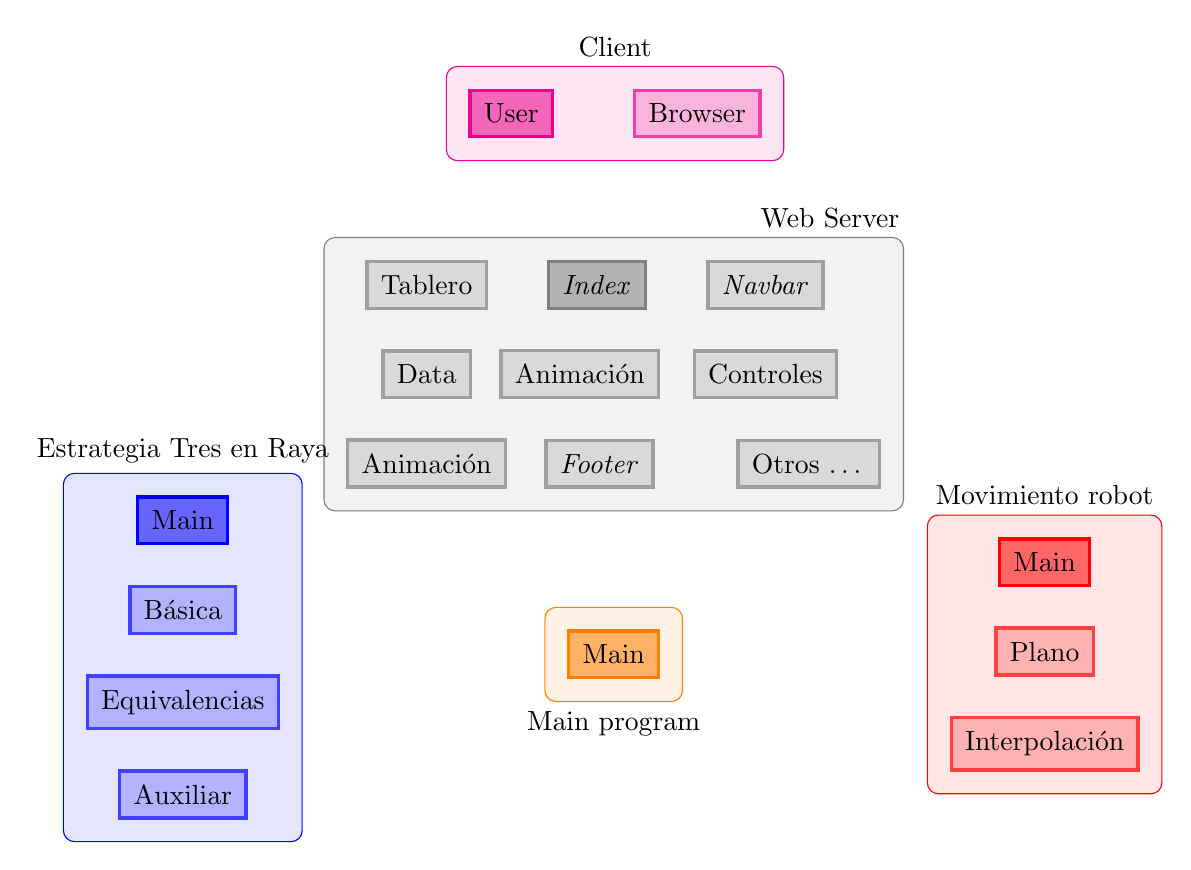
\begin{tikzpicture}[
  box/.style = {
    rectangle,
    draw = #1!75,
    fill = #1!30,
    inner sep = 5pt,
    very thick
  },
  boxp/.style = {
    rectangle,
    draw = #1,
    fill = #1!60,
    inner sep = 5pt,
    very thick
  },
  cont/.style = {
    shape = rectangle,
    align = center,
    draw  = #1,
    fill  = #1!10,
    rounded corners,
    inner sep = 8pt
  },
  con/.style = {
    -stealth,
    very thick
  }
  ]
  % Cliente.
  \node[boxp=magenta] (Us) {User};
  \node[box=magenta] (UN) [right=of Us] {Browser};
  \begin{scope}[on background layer]
    \node[fit=(Us)(UN), cont=magenta, label={Client}] (U) {};
  \end{scope}

  % Servidor Web.
  \node[boxp=gray] (SI) [below=1.25 of U, xshift=-6.5] {\textit{Index}};
  \node[box=gray] (ST) [left=.75 of SI] {Tablero};
  \node[box=gray] (SN) [right=.75 of SI] {\textit{Navbar}};
  \node[box=gray] (SD) [below=.5 of ST] {Data};
  \node[box=gray] (SA) [right=.35 of SD] {Animación};
  \node[box=gray] (SC) [below=.5 of SN] {Controles};
  \node[box=gray] (SCi) [below=.5 of SD] {Animación};
  \node[box=gray] (SF) [below=.5 of SA, xshift=.25cm] {\textit{Footer}};
  \node[box=gray] (SE) [below=.5 of SC, xshift=.55cm] {Otros \ldots};
  \begin{scope}[on background layer]
    \node[fit=(SI)(ST)(SN)(SC)(SCi)(SD)(SE)(SA), cont=gray,
    label=above right:{Web Server}] (S) {};
  \end{scope}

  % Programa Principal.
  \node[boxp=orange] (Mai) [below=1.5 of S] {Main};
  \begin{scope}[on background layer]
    \node[fit=(Mai), cont=orange, label=below:{Main program}] (Ma) {};
  \end{scope}

  % Brazo robótico.
  \node[boxp=red] (MM) [above right=.25 and 4 of Ma] {Main};
  \node[box=red] (MP) [below=.5 of MM] {Plano};
  \node[box=red] (MI) [below=.5 of MP] {Interpolación};
  \begin{scope}[on background layer]
    \node[fit=(MM)(MP)(MI), cont=red, label={Movimiento robot}] (M) {};
  \end{scope}

  % Tres en Raya.
  \node[boxp=blue] (TEs) [above left=.78 and 4 of Ma] {Main};
  \node[box=blue] (TB) [below=.5 of TEs] {Básica};
  \node[box=blue] (TEq) [below=.5 of TB] {Equivalencias};
  \node[box=blue] (TA) [below=.5 of TEq] {Auxiliar};
  \begin{scope}[on background layer]
    \node[fit=(TEs)(TB)(TEq)(TA), cont=blue, label={Estrategia Tres en Raya}] (T) {};
  \end{scope}

  % Conexiones globales.
  \connectV{U}{S};
  \connectV{S}{Ma};
  \connectH{T}{Ma};
  \connectH{Ma}{M};
\end{tikzpicture}
}
\end{frame}



\section{Chapter 7. Project Analysis}

\subsection{Planning and Scheduling}

\begin{frame}{Table of Activities}{Main activities broken down into tasks}
  \centering
  \scalebox{.75}{
    \begin{tabular}{cp{.55\textwidth}cc}
      \toprule

      \rowcolor{topRowColor}
      \textbf{Code} & \textbf{Activity} & \textbf{Start} & \textbf{End} \\
      \midrule

      \rowcolor{rowColor}
      \textbf{A} & \textbf{Learn basics of \acs{ml}/\acs{dl}}                                      & Oct. & Jan. \\
      \rowcolor{rowColor}
      A1         & \Acs{ml} course~\cite{ng20:machin_learn}                                        & -    & -    \\
      \rowcolor{rowColor}
      A2         & \Acs{dl} lectures from UPC~\cite{giro-i-nieto20:all_deep_learn_upc_etset_telec} & -    & -    \\
      \rowcolor{rowColor}
      A3         & Stanford CS231n: \acsp{cnn} for Visual Recognition~\cite{li20:cs231}            & -    & -    \\
      \rowcolor{rowColor}
      A4         & \Acs{dl} specialization~\cite{ng20:deep_learn_special}                          & -    & -.   \\
      \midrule

      \textbf{B} & \textbf{Learn thesis topic}                                                       & Dec. & Feb. \\
      B1         & Multimodal learning lectures~\cite{giro-i-nieto20:all_deep_learn_upc_etset_telec} & -    & -    \\
      B2         & Publications                                                                      & -    & -    \\
      B3         & State-of-the-art papers on \acs{rec}                                              & -    & -    \\
      \midrule

      \rowcolor{rowColor}
      \textbf{C}             & \textbf{Models creation} & Jan. & Apr. \\
      \rowcolor{rowColor} C1 & Server usage             & -    & -    \\
      \rowcolor{rowColor} C2 & Multiple iterations      & -    & -    \\
      \rowcolor{rowColor} C3 & Generate test values     & -    & -    \\
      \midrule

      \textbf{D} & \textbf{Web development}                    & Feb. & Apr. \\
      D1         & Front end (\acs{html}, \acs{css}, \acs{js}) & -    & -    \\
      D2         & \Acs{api} creation (PHP)                    & -    & -    \\
      D3         & Web server configuration                    & -    & -    \\
      D4         & Publish website (domain, server)            & -    & -    \\
      \midrule

      \rowcolor{rowColor}
      \textbf{E}             & \textbf{Bachelor's thesis}          & Dec. & May \\
      \rowcolor{rowColor}
      E1                     & Write thesis (\LaTeX)               & -    & -   \\
      \rowcolor{rowColor}
      E2                     & Create presentation slides (\LaTeX) & -    & -   \\
      \rowcolor{rowColor} E4 & Prepare presentation                & -    & -   \\
      \bottomrule
    \end{tabular}
  }
\end{frame}

\begin{frame}{Gantt Chart}{Gantt chart of main activities}
  \centering
  % -*- TeX-master: "../../Thesis.tex" -*-



\tikzset{external/export = false}
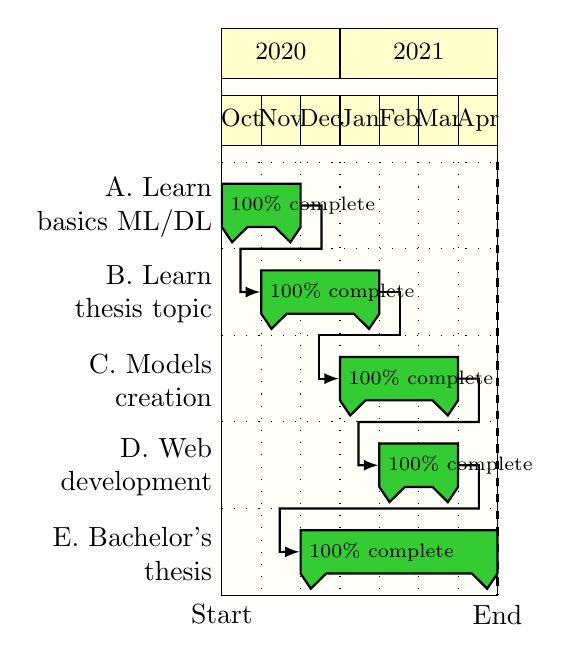
\begin{tikzpicture}
  \begin{ganttchart}[
    % Time format.
    time slot format = isodate-yearmonth,
    time slot unit = month,
    % Grid.
    vgrid = {*1{black, loosely dotted}},
    hgrid={*1{black, loosely dotted}},
    % Title.
    title/.append style = {
      fill = yellowGantt,
    },
    title height = .75,
    y unit title = .85cm,
    % Canvas.
    canvas/.append style = {
      fill = yellowGantt!15
    },
    y unit chart = 1.1cm,
    expand chart = \textwidth,
    % Today configuration.
    today = 2021-04,
    today label = {},
    % Progress style.
    progress = today,
    group progress label anchor = west,
    % Group style.
    group/.append style = {
      fill = greenGantt,
      draw = black,
      thick
    },
    group incomplete/.append style = {
      fill = greenGantt!30,
      draw = black,
      thick
    },
    group label font = \mdseries,
    group height = .5,
    group top shift = .25,
    group right shift = 0,
    group left shift = 0,
    group peaks height = .175,
    group peaks width = .65,
    group peaks tip position = .4,
    group label node/.append style = {
      align = right
    }, % Important.
    % Vertical rule (auxiliar).
    vrule/.style = {
      draw = none
    },
    % Link style.
    link/.style = {
      -latex,
      thick
    },
    link bulge = .5
    ]{2020-10}{2021-04}

    % Years and months.
    \gantttitlecalendar{year, month=shortname} \\

    % Groups.
    \ganttgroup{A. Learn\ganttalignnewline basics ML/DL}{2020-10}{2020-11} \\
    \ganttgroup{B. Learn\ganttalignnewline thesis topic}{2020-11}{2021-01} \\
    \ganttgroup{C. Models\ganttalignnewline creation}{2021-01}{2021-03} \\
    \ganttgroup{D. Web\ganttalignnewline development}{2021-02}{2021-03} \\
    \ganttgroup{E. Bachelor's\ganttalignnewline thesis}{2020-12}{2021-04}

    % Vertical rules.
    \ganttvrule{Start}{2020-09}
    \ganttvrule{End}{2021-04}

    % Group links.
    \ganttlink{elem0}{elem1}
    \ganttlink{elem1}{elem2}
    \ganttlink{elem2}{elem3}
    \ganttlink{elem3}{elem4}
  \end{ganttchart}
\end{tikzpicture}

\end{frame}


\subsection{Cost Analysis}

\begin{frame}{Title}{Subtitle}
  Hey.
\end{frame}


\subsection{Environmental Impact}

\begin{frame}{Title}{Subtitle}
  Hey.
\end{frame}



\section{Chapter 8. Conclusions}

\subsection*{}

\begin{frame}{Title}{Subtitle}
  Hey.
\end{frame}

\subsection{Future work}

\begin{frame}{Title}{Subtitle}
  Hey.
\end{frame}


\end{document}
